% Chapter Template

\chapter{Experiment Materials \& Methodology} % Main chapter title

\label{ExperimentMaterialsMethodology} % Change X to a consecutive number; for referencing this chapter elsewhere, use \ref{ChapterX}

In this paper, heavy importance is placed on primary experimental observations and data. Thus, an LSTM neural network is implemented to perform the investigation, with the use of Google’s Tensorflow machine learning API. Using this API allowed for ease of visualizing performance data and greater freedom in the network’s architecture. The network architecture will remain a control variable throughout all trials. The independent variables are the speech feature extraction algorithms, which include STFT spectrograms, Mel spectrograms, MFCCs, and DWTs. The dependent variables are the loss calculated by connectionist temporal classification (CTC) loss, word error rate (WER), and the time taken by each network when processing the test dataset. WER is calculated by the number of substitutions, insertions, and deletions divided by the number of characters and it is a more accurate metric to assess linguistic proximity than loss~\cite{wang_acero_chelba_2003}.

%----------------------------------------------------------------------------------------
%	ABSTRACT
%----------------------------------------------------------------------------------------

\section{Datasets Used}

The LJ Speech Dataset is used to train the neural network that conducted the experiment~\cite{ito_johnson_2017}. The dataset contains 13,100 NLC audio clips of around 4-8 seconds that are spoken by a single speaker reading from a selection of non-fiction literature~\cite{ito_johnson_2017}, amounting to a total of approximately 24 hours of data. 10\% of this data is used for validation while 90\% is fed into training. All in all, there is an average of ~17 words that are spoken in each ~6-second clip and there are around 13,800 distinct words said among all the audio clips~\cite{ito_johnson_2017}.

%-----------------------------------
%	PRE-PROCESSING
%-----------------------------------
\section{Pre-Processing}

The dataset provided the sound files in wav format, which made it very simple to extract its waveform data. Tensorflow’s audio analysis library in combination with PyWavelets~\cite{lee_gommers_waselewski_wohlfahrt_oleary_2019} performs each speech feature extraction algorithm on every sample in the dataset to obtain the respective input data (Figure~\ref{fig:MelSample}).

\begin{figure}[th]
    \centering
    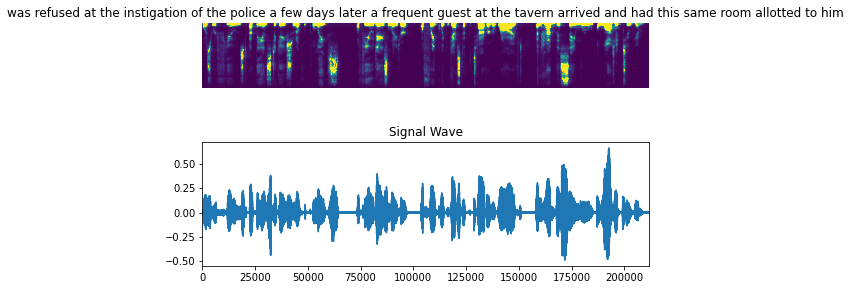
\includegraphics[width=0.9\textwidth]{Figures/melsample.png}
    \decoRule
    \caption[Mel Sample]{Sample of training data paired with its transcription, visualized as a Mel Spectrogram using Tensorflow’s signal library and its respective signal wave}
    \label{fig:MelSample}
\end{figure}

%-----------------------------------
%   NETWORK ARCHITECTURE
%-----------------------------------
\section{Network Architecture}

This report uses an end-to-end recurrent character-based neural network that consists of two convolutional layers, five layers of bidirectional LSTM cells, a dense layer, and a decoding layer to process and display the final output. The LSTM layers take in a time step of data (whose shape is dependent on the feature extraction algorithm), utilize 128 hidden units in each cell and output a one-hot matrix of shape (31, 1) at each time step. The output is a probability matrix of 31 characters that the model predicts the audio signal refers to at that point in time, which includes all of the Latin alphabet, three punctuation marks, as well as a space and a blank character. A character classification system is used over phoneme-based or word-based systems since with the current LSTM network architecture, it is capable of distinguishing between similar-sounding characters in the English dataset used. A working result of this model would output a sequence of slurred letters that, once decoded with CTC loss, would output a word; the model could output “b\_uu\_t\_  \_n\_oo”, which suggests that the original audio input is of a person uttering “but no”~\cite{graves_fernández_gomez_schmidhuber_2006,scheidl_2018}. After this procedure, these characters can be fed into an English language model to be further refined into comprehensible written text as the final output. Refer to~\autoref{AppendixC} for model details.
\par
The LSTM model is trained on 389 batches of training data with each batch consisting of 32 audio clips. The model is trained for 5 epochs for each set of independent variables, with a learning rate of 0.0001 to avoid overfitting, and evaluated by three validation datasets. Each of the three trials holds 21 batches of data that determine the accuracy of each model.
\par
Regarding the feature extraction algorithms, the MFCC trials will have 21 coefficients and the DWT trials will use a biorthogonal 6.8 wavelet (Figure~\ref{fig:MelSample}).

\begin{figure}[th]
    \centering
    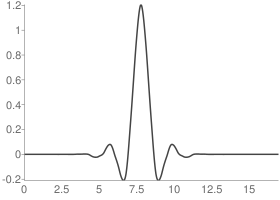
\includegraphics[width=0.5\textwidth]{Figures/wavelet.png}
    \decoRule
    \caption[Bior Wavelet]{A biorthogonal 6.8 wavelet, visualized (Source: Waselewski~\cite{wasilewski_2008})}
    \label{fig:BiorWavelet}
\end{figure}

%-----------------------------------
%	EXPERIMENTAL PROCESS
%-----------------------------------
\section{Experimental Process}

It is essential to clarify some notable semantics of this investigation. The general performance of a model within this investigation is assessed on a synthesis of its accuracy and its efficiency as well as how it compares with other models, though with the greatest emphasis on accuracy. The accuracy of a model is calculated appertaining to both its loss from CTC and its word error rate, and the efficiency of a model is gauged on a comparison of its estimated time complexity and a measured difference of time. For each speech feature extraction algorithm, there will be three trials held, amounting to a total of 4 models and 12 trials. 